\chapter{Methods\label{methods}}
This chapter aims to establish a precisely defined and rigorous research approach to enhance transparency and repeatability. We will take the steps required to ensure that every phase and decision is thoroughly documented, enabling the reader to retrace the research process. In a thesis made by a single researcher the lack of cross-examination of results with multiple researchers and the validation of evaluation criteria for opinion bias pose threats to validity, as will be clarified further in \hyperref[discussion]{Chapter 4}. Therefore, special attention will be paid to address these concerns. By following this approach, this research endeavors to contribute to the existing body of knowledge in the field of computer science in a robust and reliable manner.

\textcolor{red}{stage 1 licenses amount before rough deduplication could be a nice metric to say for my excel efforts. duplicates.txt can be just a one-time pass of the difflib duplicate thingy. ok now ill go through once the excluded and included licenses one by one and note any broader scale "mistakes" in the search string. gotta add sources on top of source}

\textcolor{red}{at the end of this section i will have to document the timestamp at which point i accessed the docs of scancode-licesendb since. actually i might be a good idea to create a wayback machine attempt to capturing the state of the licensedb rn. nvm great wayback machine is not viable solution for that. just stating here that i downloaded the licensedb on 2025 mar 25 15:30}

\textcolor{red}{it's good to note that when bumping into the missing license of attpubliclicense which was from gnu, it turned out that the license listing site doesnt state the license content whatsoever. i had to just put the comment of the license into manual licenses.}

\textcolor{red}{manual/missing licenses: check which shortcodes of missing licenses does stage2-3.py output. check from sheets where does the shrotcode originate from. ctrl + f that listing site. copy the full license to manual-licenses/shortcode.txt and re-run the stage2-3.py until no longer missing licenses appear in console.}

\textcolor{red}{remember to count here how many missing licenses / manual licenses had to be done manually}

\textcolor{red}{could be also a good idea to note here how many missing licenses came from which site. gnu and fsf seem to be the winners here.}

\textcolor{red}{cvw was not found with the python script. i checked from the excel that its from the osi but osi didnt have it anymore by the time i got there. at some point between fetching the data and the re-fetching the license content from the original site MITRE had voluntarily retired the cvw license. it was found from the scancode licensedb with the name cvwl instead. dejavu and dbg-3.0 were also two other licenses that contained a space. this might indicate that the space is an accident that its simply just not found from a license listing site x. its also good to note that the python script was decided to be an valid approach since many of the licenses were actually found with the shortcode from the licensedb scancode. fetching 700 licenses by hand would have had time and validity issues. wayback machine could have been used to do the actual searching as well. this is unfortunately a validity issue but at least the source is available in wayback machine.}

\textcolor{red}{let it be said, that when looking for manual licenses, if there existed two sites which listed the same license, the leftmost was chosen, as per the order of the wikipedia mit article}

\textcolor{red}{it seems like i have manually added licenses and invented shortcodes for them AT LEAST in DFSG license listing. FAL is a good example.}

\textcolor{red}{For example licenses like CorkForkPL from FSF are just empty licenses. CorkForkPL is used however in MighTyD project but the license would have to be seen from a downloaded project or something like that. A new scope: only licenses that are one (1) click away from the initial license landing page can be copypasted to the manual licenses. just like the JahiaCSL has a URL on FSF for the license new location although the FSF page is empty.}

\textcolor{red}{licenses like MPL exist on FSF and GNU. it was not easily found from FSF (empty with links to programs using this) so it was gotten from GNU which was labeled as MPL1.1, which the FSF DOES have so i just boldly went with that. threat to validity.}

\textcolor{red}{it could be a good idea to mention how many missing licenses came out of which sites. or it could be out of scope. i can just make a validity threat and say with face value that most of them were from FSF, GNU in that order. Python license seems just straight up an accident on FSF's side. scope is not to fix the documentation problems of the 5 organizations though so I'll leave it just like that and mention the possibility of it being just an accident.}

\textcolor{red}{so. now i figured ill take another validity threat L and decide to remove duplicates by human eyesight and choose the one left over from two seeming duplicates by pure human eyesight. i will document the ones that were chosen over the other duplicate and call it a day. for now. i gotta write number + shortcode to find duplicates and document them.}

\textcolor{red}{it would be good to note in conclusions that while im stripping away here the errorish licenses and "duplicates". the ones used mostly are different from those that are actually legally valid historically or even those that are not meant to be legally valid (MIT). whilst im doing this systematically it doesnt mean that all parts of it can be done automatically or by automation. human touch in for example checking the incl excl criteria and removing duplicates by combining and creating the weight value of shortcode + license name + license text is done basically by a human with the help of python first sorting them based on their word overlap (not sort, not full on difflib, not cosine similarity). ill do exclusion first though. inclusion is kinda implied here i just realized when i took them out of the license listing cites and removed blanks etc.}

\textcolor{red}{is a documentation license a software license. ok with the initial beginning inclusion words \\"(source|software|program|code|module|public(s+)license|ware|(w+)ware)" we managed to catch GFDL licenses and for this scope i think ill have to narrow it down to just purely source code or software targeting licenses. then again is font a piece of software. documentation might not be. font is considered a software in this scope of ours since the fonts might contain programmatic instructions how to draw and render them. documentation might be a part of a software package but is not considered software regardless.}

\textcolor{red}{i will call it a day to just remove creative commons licenses by exclusion string and remove GFDL licenses by manually providing a list of excluded licenses. the point of this thesis and this research is to provide how many public software licenses do we actually have so that we can understand the problem of open source and the reason why post-open source has begun to emerge. now i gotta just exclude and include (in that order) then just very lightly and cheaply remove the duplicates by checking licenses one by one with difflib}

\textcolor{red}{how do i exclude documentation from here do i need to manually exclude them? i can always just call it a day on validity threat and change it afterwards???? i started with}

% r'^(?!.*\b(documentation\s+license|creative\s+commons)\b).*?\b(source|sources|software|program|programs|code|module|public\s+license|ware|\w+ware)\b'
\textcolor{red}{but soon realized that the point of this thesis is to provide a clearer picture of the actual problem that im trying to diminish here: the huge amount of open source licenses that exist. instead im removing everything else but the documentation license and creative commons thingy from the search string. will go through the excluded licenses once more just to check if it caught anything wrong. the big idea here is that because the open source licenses and the public licenses used are already sometimes too vague to be legally valid should be just left as is and just remove the sort of licenses that are already specifically not-software specific, i.e. documentation licenses, or at least creative commons is not considered as such.}

\textcolor{red}{the eye-pass of 87 excluded licenses included cal1.0 and cal-combined which seem to need to be included. made inclusions.txt to manually include them although containing the words creative commons, since those license texts were licensed themselves with creative commons. will eyeball the stage-2 shortcodes as well just to see anything i know by heart is not public software license. cc-by-sa-japanese was included so i had to make a manual exclusions.txt to manually mark licenses that are not public software licenses.}

\textcolor{red}{stage 2: inclusion and exclusion is done. 656 licenses left to remove potential duplicates from using ratcliff and obershelp. then just writing. literally just writing after this.}

\textcolor{orange}{so for stage 2: i output shortcodes to .txt and full licenses to folder. from .txt i bake them to google sheets and match the sources for them. from google sheets i put them to github markdown for reader to see. note: the python script does not work on windows due to some path handling errors. i would have loved to use my desktop 1160K instead of laptops i5-8265U. ok wow it took 4101.285 seconds on my laptop. check the ss on my laptop}

\textcolor{orange}{licenses texts were sorted using difflib and renamed index plus shortcode. then opened in vscode and if seem the same content minus noise the other one usually the order of the 5 licnse sites is removed as duplicate. vscode compare tool was used to help with larger license texts. data/database licenses popped up during the duplicate searching phase. added ad-hoc open data as an exclusion string}

\textcolor{orange}{duplicate removal in tabs was done so that: i check the text if the n and n+1 and if they look pretty much the same i act and if the shortcodes look the sam i act.}

\textcolor{red}{stage 3 is removing duplicates by a feel factor from the shortcodes and from the difflib sorted contents. this is also just a one pass test.}

The systematic literature review method is a well-established approach for conducting a comprehensive and rigorous analysis of the existing research on specific research question or subject \citep{kitchenham2007}. This paper presents a multivocal literature review. Multivocal literature review is type of systematic literature review that includes both academic literature and grey literature \citep{mantyla2019}. This method was selected for this study to facilitate a thorough and scientifically interdisciplinary examination of public licenses in software engineering. The existing literature consists of public software licenses not found in academic databases and as such are considered gray literature, making the thesis a multivocal literature review.

This study follows the guidelines outlined by \cite{kitchenham2007}, to ensure its quality. The multivocal review method consists of three distinct phases: planning, conducting and reporting the review. This study stricly adhered to this structure. The phases can be further broken down into a research protocol, as illustrated in \hyperref[fig:slrphases]{Figure 2.1}. Adhering to the protocol is the first step in ensuring a well-documented and rigorous process, which increases the validity and auditability of the study.

\begin{figure}
	\centering
	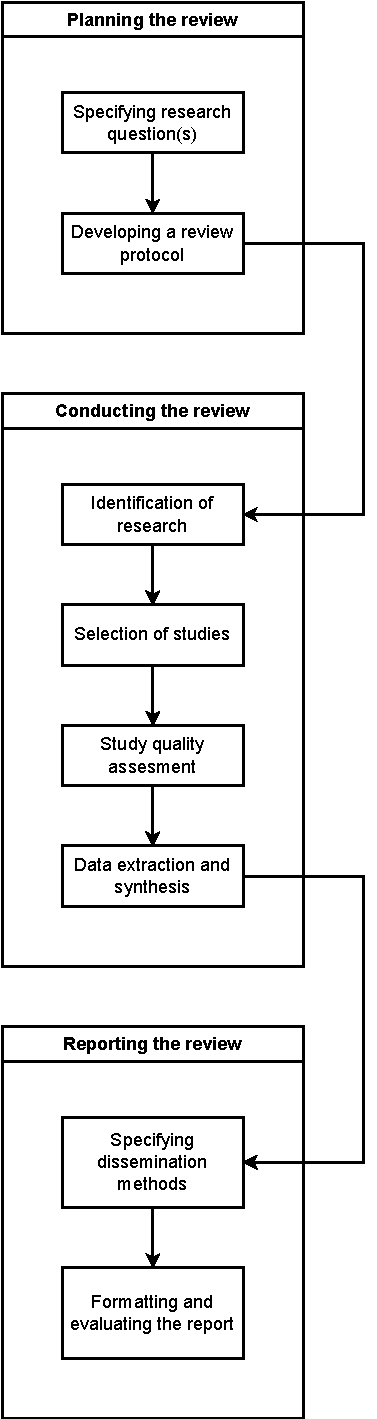
\includegraphics[scale=0.9]{figures/slr-phases.pdf}
	\caption{Three phases of a systematic literature review}
	\label{fig:slrphases}
\end{figure}

The multivocal literature review process began with the formulation of research questions and the establishment of a comprehensive search strategy and scope. The search process was conducted by employing a quasi-gold standard (QGS) approach based on the implementation by \cite{qgs}. After the completion of the search process, the inclusion and exclusion criteria were defined. To ensure a structured evaluation of the literature, a data extraction form was created. Finally, a strategy for analyzing the extracted data from the literature was designed.

 To ensure the reliability and validity of the research protocol, it was validated against similar systematic literature reviews in computer science, the aforementioned guidelines by \cite{kitchenham2007}, and was further refined through an iterative process. Specifically, a subset of the data was tested on (The QGS) and any identified issues or problems were recorded and addressed. The details of this process are explained and thoroughly documented in the following sections. Similarly, the same approach was followed for the data extraction process, whereby a subset of literature was tested to refine the data extraction form. The revision of the form was undertaken as necessary to guarantee the completeness and accuracy of the extracted data.

\section{Research questions}
The research questions in this study served two primary purposes. Firstly, they aimed to provide an anaylsis of the existing multivocal literature on public licenses in software engineering for the researchers interested about the field. Secondly, the questions were designed to cater a secondary audience of professional software engineering practicioners. As discussed in the \hyperref[intro]{Chapter 1}, the following research questions were addressed in this thesis:

\begin{itemize}
	\item RQ1: How many public software licenses are there in the top five software license listing cites?
	\item RQ2: How much is there disagreement in the shortcode names between different public software licenses listing sites?
	\item RQ3: How many public licenses in software engineering does there exist?
\end{itemize}

The multivocal literature review in this thesis begins with addressing RQ1, which aims to provide the amount of public software licenses that exist in our five public license listing sites, per site. The review takes into account attributes like versions, supersedences to a different license family, formal or otherwise and recognizability. These attributes give us different amounts to existing PCLs in software engineering. This informatin could be most valuable to the researchers. The results can be used to introduce some notable background of the current public licenses in software engineering and enabling focus to more specific areas inside the topic of this thesis.

Next RQ2 seeks to find the amount of duplicate licenses between the license listing sites. Results to this research question are also mostly useful to researchers of the field. Moreover the documented methods are most likely the most valuable information for the researchers.

Finally RQ3 attempts to count the total number of individual public software licenses within the scope of this thesis. The research question builds on top of the results and methods of the previous research questions. This information could be most valuable for the practicioners since it could give some overview and a sense of the scale when picking a public software license that would serve the practicioners' needs the best.

% where was search process conducted in (inclusion/exclusion in appendix a)
\section{Search stragey}
The search process was conducted on five public license listing websites. The selection criteria for the literature were defined after the search process and the selection process was based on inclusion and exclusion criteria. The inclusion and exclusion criteria and each step of exclusion on the literature found are presented later in this chapter.

% data extraction process
The data extraction process was performed in a standardized and systematic manner, with the aim of obtaining the relevant information from the selected literature. The data extraction form used included license shortcode used in the listing site, listing site name, full license text and is available  \hyperref[table:extraction]{Table 2.2}. The extracted data was then used to answer the research questions and perform the data analysis. The results of the data analysis were then reported in a rigorous manner.

% - more on where was search process conducted in
\subsection{Search method}
The search was conducted on five license listing websites, as mentioned earlier, to obtain a broad set of multivocal literature. This approach yielded a large number of literature that were processed to a subset of high-relevance literature using exclusion and quality criteria presented later in this chapter. Manual searching of databases with hundreds of public licenses is not feasible, and it is prone to researcher bias and may overlook relevant venues from other scientific disciplines. However, a preliminary manual search was performed to reduce the number of iterations required and establish the quasi-gold standard (QGS) mentioned earlier.

% how were search terms determined (end condition)
\subsection{Search scope and terms}
Originally the search terms would have been present just like in a normal multivocal literature review or in a systematic literature review. Keywords however produced highly varying and non-reproducabe results in Google Scholar and Google Search. Some PCL listing websites such as FSF's list of pages categorized as licenses could not be found from Google Search even with the \texttt{site} operator: \\
\texttt{site:https://directory.fsf.org/wiki/Category:License}. Although the page has been up since 2013, for some reason Google has not crawled the page in 10 years \citep{fsf:licenselist}. Hence why this thesis does not include search terms of the initial phase per se but rather inclusion and exclusion strings on the second phase.

% inc-exc string
The inclusion and exclusion string was established on a basis of quasi-gold standard as proposed by \cite{qgs}. For establishing a QGS we employed a manually crafted inclusion and exclusion string based on the topic and research questions of this study. As we defined public licenses in software engineering as licenses where the licensees are not limited and the license in question is meant be used in licensing software source code in \hyperref[intro]{Chapter 1} and our research questions focus on finding useful metrics about the public licenses, we manually formulated the inclusion and exclusion string we decided to gather PCLs from the related web pages of the aforementioned categorizers: SPDX, FSF, OSI and GNU.
Instead, for establishing a QGS we started defining our search scope from the Wikipedia page of one of the most used open source license according to \cite{github:licenseusage}, the MIT license \citep{wikipedia:mit}. The infobox contained fields in the order shown in \hyperref[table:infobox]{Table 2.1}.

\begin{table}[t]
	\begin{center}
		\begin{tabular}{||c c||}
			\hline
			Field & Value \\
			\hline
			Publisher & Massachusetts Insitute of Technology \\
			SPDX identifier & MIT \\
			Debian FSG compatible & Yes \\
			FSF approved & Yes \\
			OSI approved & 	Yes \\
			GPL compatible & Yes \\
			Copyleft & No \\
			Linking from code with a different license & Yes \\
			\hline
		\end{tabular}
		\caption{MIT License Wikipedia page infobox}
		\label{table:infobox}
	\end{center}
\end{table}

% how many results
As we defined public licenses in software engineering as licenses where the licensees are not limited and the license in question is meant be used in licensing software source code in \hyperref[intro]{Chapter 1} and our research questions focus on finding measurements and reasonings to the PCLs' various attributes, we decided to gather PCLs from the related web pages of the aforementioned categorizers: SPDX, FSF, OSI and GNU. The publisher, GPL compatibility, copyleft and the linking exception did not result in any meaningful PCL listing websites. This leaves us with the SPDX, Debian FSG compatibility, FSF and OSI from which all resulted in some sort of PCL listing websites.

With the search for the initial PCL listing websites completed we moved onto the search process itself.

\section{Search process}
The literature selection process was divided into multiple stages, as outlined in \hyperref[fig:search-process]{Figure 2.2}. The initial step involved the formation of the first PCL listing websites through which the first literature would be acquired from.

\begin{figure}
	\centering
	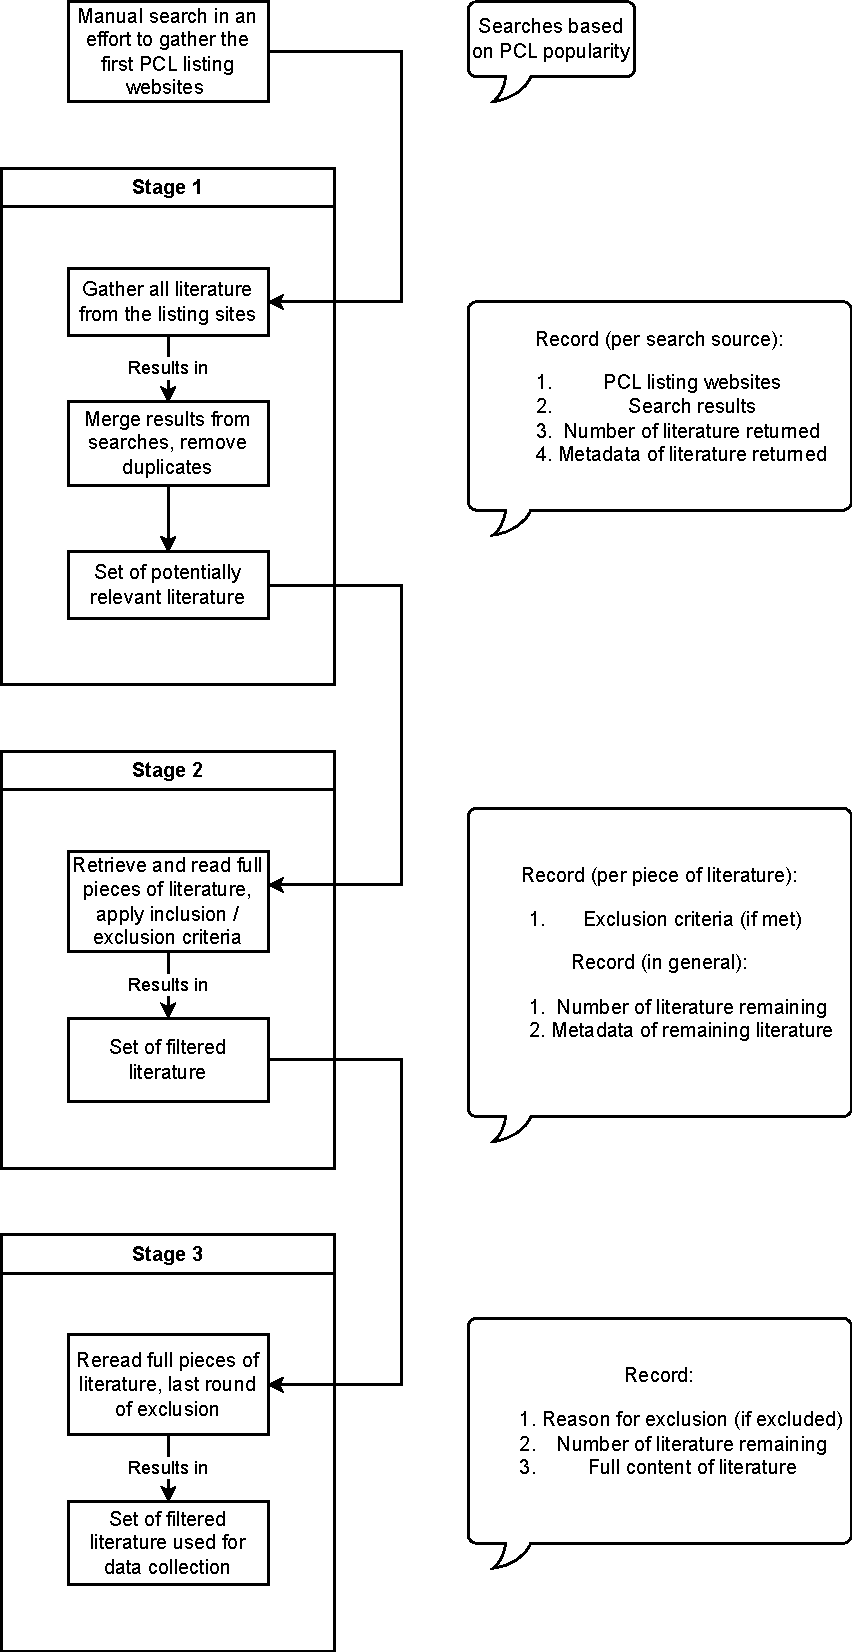
\includegraphics[scale=0.67]{figures/search-process.pdf}
	\caption{Search process divided into stages}
	\label{fig:search-process}
\end{figure}

\textcolor{red}{does this figure 2.2 have to use these terms since im really just applying K \& C 2007 slr guidelines to a mlr. no it doesnt. change it when finishign up 2. methods.}

In the first stage, the search was conducted using the ''SPDX License List'' \citep{spdx:licenses}, ''The DFSG and Software Licenses'' \citep{debian:dfsg}, FSF's ''Category:License'' Wiki page \citep{fsf:licenselist}, GNU's ''Various Licenses and Comments about Them'' \citep{gnu:licenselist} and "OSI Approved licenses" \citep{osi:licenselist}. The PCLs appear in the same order as decribed above: SPDX, DFSG, FSF, OSI and GNU. The appendix was also crafted in a spreadsheet software so that only the initial hit source was documented in the order described above. For example even if MIT license would be found on SPDX and DFSG \hyperref[appendix:a]{Appendix A} would only display MIT license with the ''First hit from'' value being SPDX. The initial list of 789 PCLs excluding duplicates is provided in \hyperref[appendix:a]{Appendix A}. %cite mscthesis github repo here

Some things must be mentioned about the process of the first stage. First, the FSF outputted a ''license'' named ''other''. This ''license'' included at the time of observation 5282 known programs to FSF whose PCLs were not documented yet by the FSF. Although some of the programs had straightforward PCLs such as GPL-2.0-only we decided to leave these PCLs out of the scope of this thesis due to the large amount of the programs. The second note is about GNU's PCLs. Since we had the most trouble scraping the identifiers automatically from this website we decided to limit the PCLs only to ''Software Licenses'' as defined by the table of contents on the website.

\textcolor{red}{approx duplicates were the result of going to the two listing websites that had the approaximately same looking licenses. then i just checked if they were actually some sort of duplicates of one another or if they already exist somewhere else. examples here. this is also a validity threat. problem with focusing software specific licenses is for example wtfpl. it is mostly used in software licensing but it doesn't quite clearly state that it is software specific license. maybe ill have to include the word "public license" and just include stuff that's not actually software specific or maybe ill make some exclusion criteria in order to get less non-software licenses}

In the second stage, the inclusion and exclusion criteria were applied to further filter the literature and reduce the number of licenses to be reviewed. This involved a manual review of the full licenses. The exclusion reason as a shortcode (e.g. I1 = failed to meet inclusion criteria 1 or E2 = met exclusion criteria 2) is provided in \hyperref[appendix:b]{Appendix B}.

The third stage was the most time-consuming and involved a manual review of the full licenses. After reading and evaluating each license, a final round of exclusions was completed and documented. The remaining licenses were used for data collection and analysis in the final part of the study. The final list of licenses is available in \hyperref[appendix:A]{Appendix A}.

\section{Inclusion and exclusion criteria}
To be eligible for the data collection and analysis, a license had to meet all of the following inclusion criteria:

\begin{itemize}
	\item I1: The license focuses on the copyright of software source code or their binaries
	\item I2: \textcolor{red}{inclusion criteria 2}
\end{itemize}

Additionally, licenses were excluded if they met any of the following criteria:

\begin{itemize}
	\item E1: The piece of literature is a license exception
	\item E2: The piece of literature is a Creative Commons license
	\item E3: \textcolor{red}{exclusion criteria here}
	\item E4: \textcolor{red}{exclusion criteria here}
\end{itemize}

The relevance of each piece of literature was evaluated based on inclusion and exclusion criteria stated above. In cases where there was doubt about the suitability of a license, a more in-depth manual examination of its content was performed. The reason for exclusion was documented for each license that failed to meet the criteria, and when it was unclear, the license was included by default.

Another relevant criteria related to the ones of inclusion and exclusion are the quality and evidence criteria. These criteria used by \cite{dyba2007} were not put into practice in this thesis since individual PCLs per se might not be meaningful in a results, evidence nor quality perspective. This puts more emphasis on the inclusion and exclusion criteria so that is something we must be mindful about.

\section{Data collection and data analysis}
To answer the research questions of this thesis, a thorough examination of the selected primary literature was conducted and the necessary data was collected using data extraction form presented in \hyperref[table:extraction]{Table 2.2}. A record of extracted data was kept for anaysis and is available as \hyperref[appendix:b]{Appendix B}.

\begin{table}[t]
	\begin{center}
		\begin{tabular}{||c c c||} 
			\hline
			\# & Field & Concern/Research question \\
			\hline
			F1 & Shortcode & RQ2, RQ3 \\
			F2 & Listing site name & RQ1, RQ2 \\
			F3 & Full text &  Documentation\\
			\hline
		\end{tabular}
		\caption{Data extraction form}
		\label{table:extraction}
	\end{center}
\end{table}

The subsequent chapter presents the outcomes of the steps taken in the study, as discussed above.